\documentclass[10pt,a4paper]{article}
\usepackage[utf8]{inputenc}
\usepackage[margin=1in]{geometry}
\usepackage{amsmath,amssymb,amsfonts}
\usepackage{chemfig}
\usepackage{tikz}
\usepackage{pgfplots}
\usepackage{enumitem}
\usepackage{fancyhdr}
\usepackage{booktabs}

\pgfplotsset{compat=1.18}

\pagestyle{fancy}
\fancyhf{}
\rhead{USNCO 2025 National Exam Part II}
\lhead{ID Number: \underline{\hspace{3cm}}}
\rfoot{Page \thepage}

\begin{document}

\begin{center}
    \large\text{2025 U.S. NATIONAL CHEMISTRY OLYMPIAD NATIONAL EXAM PART II} \\
    \vspace{0.2cm}
    \normalsize\text{Prepared by the American Chemical Society Chemistry Olympiad Examinations Task Force}
\end{center}

\vspace{0.5cm}

\subsection*{Question 1}
\textbf{1. [12\%]} Copper(II) sulfate pentahydrate, $\text{CuSO}_4\cdot5\text{H}_2\text{O}$, is a blue crystalline solid. Upon gentle heating, it loses water to form anhydrous $\text{CuSO}_4$, which is a white solid.

\begin{enumerate}[label=\alph*.]
    \vspace{5cm} \item When 5.000 g $\text{CuSO}_4\cdot5\text{H}_2\text{O}$ is heated to remove all of its water, what mass of anhydrous $\text{CuSO}_4$ will be produced?
    \vspace{5cm} \item Explain the change in color on dehydration of $\text{CuSO}_4\cdot5\text{H}_2\text{O}$.
    \vspace{5cm} \item A solution of 0.0506 g $\text{Cu}(\text{CH}_3\text{COO})2\cdot\text{H}_2\text{O}$ is made up with water to a volume of 5.00 mL water. This solution in a 1-cm cuvette produces the visible spectrum shown. What wavelength would be the best choice to determine the concentration of $\text{Cu(II)}$?
    
    \begin{center}
    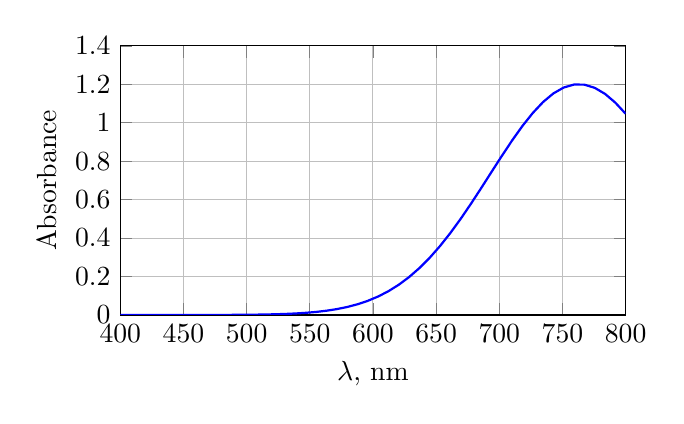
\begin{tikzpicture}
    \begin{axis}[
        width=8cm, height=5cm,
        xlabel={$\lambda$, nm},
        ylabel={Absorbance},
        xmin=400, xmax=800,
        ymin=0.0, ymax=1.4,
        xtick={400,450,500,550,600,650,700,750,800},
        ytick={0.0,0.2,0.4,0.6,0.8,1.0,1.2,1.4},
        grid=both
    ]
    \addplot[blue, thick, domain=400:800, samples=50] {1.2*exp(-((x-763)/100)^2)};
    \end{axis}
    \end{tikzpicture}
    \end{center}

    \vspace{5cm} \item A student determines the value of n in an unknown crystalline hydrate of copper(II) nitrate, $\text{Cu}(\text{NO}_3)_2\cdot n\text{ H}_2\text{O}$, by preparing 5.00 mL of an aqueous solution of a known mass of the compound and measuring its absorbance at the wavelength determined in part c. However, the student inserts the cuvette into the spectrophotometer without first wiping fingerprints from it. How will this affect the value of n determined in the experiment?
    \vspace{5cm} \item An alternative method for determining the degree of hydration of the copper nitrate is to allow a known mass of compound to react with excess KI solution, which produces a yellow-brown suspension. Write a balanced net ionic equation for this reaction.
    \vspace{5cm} \item The experiment in part e is carried out with 0.1000 g of the hydrated copper(II) nitrate. To the resulting mixture is added a 0.0250 M solution of sodium thiosulfate, $\text{Na}_2\text{S}_2\text{O}_3$, until the color of the mixture has just dissipated, leaving a milky white suspension. This requires 17.20 mL of added sodium thiosulfate solution. What is the value of n for the $\text{Cu}(\text{NO}_3)_2\cdot n\text{ H}_2\text{O}$?
\end{enumerate}

\subsection*{Question 2}
\textbf{2. [13\%]} Calcium oxalate, $\text{CaC}_2\text{O}_4$ has a $K_{sp}$ of $2.7\times10^{-9}.$ Oxalic acid, $\text{H}_2\text{C}_2\text{O}_4,$ has two ionizable hydrogens with $pK_{a1}= 1.27$ and $pK_{a2}=4.28.$
\begin{enumerate}[label=\alph*.]
    \vspace{5cm} \item Draw a Lewis structure for oxalate ion, $\text{C}_2\text{O}_4^{2-}$, including all bonds, lone pairs, and formal charges.
    \vspace{5cm} \item Calculate the molar solubility of calcium oxalate in pure water.
    \vspace{5cm} \item Calculate the molar solubility of calcium oxalate in a 0.100 M $\text{CaCl}_2$ solution.
    \vspace{5cm} \item A 0.100 mol sample of solid $\text{CaC}_2\text{O}_4$ is suspended in 1.00 L of water and HCl(g) is bubbled through the solution until all of the solid just dissolves. What is the pH of the final homogeneous solution? You may assume the final volume of solution is 1.00 L.
    \vspace{5cm} \item How many moles of HCl(g) are added in part d?
    \vspace{5cm} \item Will the molar solubility of $\text{CaC}_2\text{O}_4$ in 0.1 M $\text{NaHC}_2\text{O}_4$ be significantly greater than, significantly less than, or within 10\% of the molar solubility of calcium oxalate in pure water? Justify your answer.
\end{enumerate}

\subsection*{Question 3}
\textbf{3. [12\%]} N,N-Dimethylethanolamine (($\text{CH}_3)_2\text{NCH}_2\text{CH}_2\text{OH}$, DMEA, $M=89.14$) is a Brønsted base whose conjugate acid, $\text{DMEAH}^+$, has a $pK_a=9.22$ ($K_a=6.0\times10^{-10}$). Acetic acid ($\text{CH}_3\text{COOH}$, $M=60.05$) has a $pK_a=4.75$ ($K_a=1.8\times10^{-5}$).
\begin{enumerate}[label=\alph*.]
    \vspace{5cm} \item Calculate $\Delta G^\circ_{rxn}$ at 298 K for the acid-base reaction of DMEA with $\text{CH}_3\text{COOH}$.
    \vspace{5cm} \item A solution consisting of 7.84 g $\text{CH}_3\text{COOH}$ and 107.17 g water is placed in a well-insulated (Dewar) flask. To this solution is added DMEA in small portions. After each portion of DMEA is added, the solution is stirred and the temperature measured with a digital thermometer. Calculate $\Delta H^\circ_{rxn}$ for the reaction of DMEA with $\text{CH}_3\text{COOH}$. You may assume that all solutions have the same specific heat capacity as pure water.
    \vspace{5cm} \item Calculate $\Delta S^\circ_{rxn}$ for the reaction of DMEA with $\text{CH}_3\text{COOH}$.
    \vspace{5cm} \item The $\Delta S^\circ$ calculated in part c. is negative. What features of the reaction of DMEA with $\text{CH}_3\text{COOH} $ cause it to have a negative entropy of reaction?
\end{enumerate}

\subsection*{Question 4}
\textbf{4. [12\%]} A galvanic cell is set up as follows and the cell potential measured as a function of temperature to give the graph shown.
\begin{enumerate}[label=\alph*.]
    \vspace{5cm} \item Which electrode is the anode and which is the cathode?
    \vspace{5cm} \item The standard reduction potential for $\text{Zn}^{2+}(aq)$ at 298 K is $-0.762$ V. What is the standard reduction potential for $\text{Pb}^{2+}(aq)$ at 298 K?
    \vspace{5cm} \item What are $\Delta G^\circ$ (at 298 K), $\Delta H^\circ$, and $\Delta S^\circ$ for the reaction shown below?
    $$\text{Zn}(s)+\text{Pb}^{2+}(aq)\rightarrow \text{Zn}^{2+}(aq)+\text{Pb}(s)$$
    \vspace{5cm} \item Explain the sign of $\Delta S^\circ$ for the reaction given in part c.
    \vspace{5cm} \item The temperature-dependence of the cell is remeasured with the same cell, except that the concentration of $\text{Pb}^{2+}(aq)$ in the left-hand compartment is changed to 0.100 M. Plot the results on the graph shown below (with the results shown from the standard cell given again for reference), and briefly justify your plot.
\end{enumerate}

\subsection*{Question 5}
\textbf{5. [12\%]} Write net equations for each of the reactions below. Use appropriate ionic and molecular formulas and omit formulas for all ions or molecules that do not take part in a reaction. Write structural formulas for all organic substances, and clearly show stereochemistry where relevant. You need not balance the equations or show the phases of the species.
\begin{enumerate}[label=\alph*.]
    \vspace{5cm} \item Carbon dioxide is bubbled through a saturated solution of barium hydroxide.
    \vspace{5cm} \item Potassium permanganate is mixed with iron(II) sulfate in dilute sulfuric acid.
    \vspace{5cm} \item Solid silver chloride is added to concentrated aqueous ammonia.
    \vspace{5cm} \item Phosphorus trichloride reacts with potassium chlorate.
    \vspace{5cm} \item Para-xylene (1,4-dimethylbenzene) is heated with a mixture of concentrated nitric and sulfuric acids.
    \vspace{5cm} \item Fluorine-18 emits a positron.
\end{enumerate}

\subsection*{Question 6}
\textbf{6. [13\%]} Oxygen has two stable allotropes, $\text{O}_2$ (dioxygen) and $\text{O}_3$ (ozone).
\begin{enumerate}[label=\alph*.]
    \vspace{5cm} \item Explain why $\text{O}_2$ has a higher normal boiling point than either $\text{N}_2$ or $\text{F}_2$.
    \vspace{5cm} \item Explain why both atomic oxygen (O) and $\text{O}_2$ have two unpaired electrons in their ground states.
    \vspace{5cm} \item Molecular oxygen has an excited state with no unpaired electrons, which emits light with a wavelength of 1270 nm to return to the ground state. What is the energy (in $\text{kJ mol}^{-1}$) by which the excited state is higher than the ground state?
    \vspace{5cm} \item Explain why $\text{O}_2$ does not absorb light in the infrared region of the electromagnetic spectrum but $\text{O}_3$ does.
    \vspace{5cm} \item Dioxygen can be oxidized to form dioxygenyl cation ($\text{O}_2^+$) or reduced to form superoxide ion ($\text{O}_2^-$) or peroxide ion ($\text{O}_2^{2-}$), while ozone can be reduced to form ozonide ion ($\text{O}_3^-$). Fill in the table below by assigning the correct distances to the six species, and briefly justify your assignments. (You may consider 127 and 128 pm as essentially the same in this problem.)
\end{enumerate}

\subsection*{Question 7}
\textbf{7. [14\%]} Cesium lead iodide, $\text{CsPbI}_3$, is of interest in solar photovoltaic cells. It adopts a structure called a perovskite whose cubic unit cell is shown below.
\begin{enumerate}[label=\alph*.]
    \vspace{5cm} \item Which element corresponds to the small gray spheres, which to the medium sized white spheres, and which to the large black spheres?
    \vspace{5cm} \item Describe the coordination number and the identity of the nearest neighbor atoms for each of the types of atoms in $\text{CsPbI}_3$.
    \vspace{5cm} \item The length of the unit cell edge in $\text{CsPbI}_3$ is 628 pm. What is the density of $\text{CsPbI}_3$ in $\text{g cm}^{-3}$?
    \vspace{5cm} \item A mixed-metal oxide that is of interest in high-temperature superconductivity research, $\text{YBa}_2\text{Cu}_3\text{O}_7$, adopts a structure related to the perovskite structure. Identify which elements correspond to the four types of spheres in the diagram.
    \vspace{5cm} \item Give the oxidation numbers of each element in $\text{YBa}_2\text{Cu}_3\text{O}_7$.
    \vspace{5cm} \item The atoms represented by the black spheres have two different coordination geometries in the structure shown. What are the geometries? How is this observation related to the oxidation numbers you determined in part e?
\end{enumerate}

\subsection*{Question 8}
\textbf{8. [12\%]} Many organic compounds react with elemental halogens such as $\text{Br}_2$ or $\text{I}_2$.
\begin{enumerate}[label=\alph*.]
    \vspace{5cm} \item Under appropriate conditions, 3-methylpentane will react with $\text{Br}_2$ to form a single monobromide with the formula $\text{C}_6\text{H}_{13}\text{Br}$. Give appropriate reaction conditions and the structural formula of the product.
    \vspace{5cm} \item Cyclohexene forms different products when reacted with $\text{Br}_2$ in water than when reacted in carbon tetrachloride. Give structural formulas for the products formed in the two solvents, including stereochemistry if relevant.
    \vspace{5cm} \item Benzene reacts with bromine in the presence of a Lewis acid catalyst. Give an example of a suitable catalyst and the structural formula of the major organic product of the reaction.
    \vspace{5cm} \item Cyclopentanone reacts with excess bromine in the presence of base to give a tetrabromide. Give a structural formula for the product and explain why the reaction does not give good yields of a monobromide product even when only one equivalent of $\text{Br}_2$ is used.
    \vspace{5cm} \item Acetophenone, $\text{C}_6\text{H}_5\text{COCH}_3$, reacts with excess iodine in the presence of aqueous sodium hydroxide to give a yellow precipitate and a water-soluble organic species. Give structural formulas for these two products.
\end{enumerate}

\newpage
\subsection*{2025 USNCO Part 2 SOLUTIONS}

\textbf{1.}
\begin{itemize}
    \item[a.] $M$ of $\text{CuSO}_4\cdot5\text{H}_2\text{O} = 249.70$, $M$ of $\text{CuSO}_4 = 159.62$. \\
    $(5.00\text{ g CuSO}_4\cdot5\text{H}_2\text{O})/249.70\text{ g mol}^{-1} = 2.002 \times 10^{-2}\text{ mol}$. \\
    $2.002 \times 10^{-2}\text{ mol} \times 159.62\text{ g mol}^{-1} = 3.196\text{ g}$ anhydrous $\text{CuSO}_4$.
     \item[b.] Copper(II) is $d^9$ and is expected to show (weak) absorption of light regardless of its environment. Dehydration of copper(II) sulfate results in a change of ligands from water ligands to sulfate ligands. The blue color is due to absorption of red light at the extreme low-energy end of the visible spectrum. The change to the (weaker-field) sulfate ligands reduces the energy of the absorption into the near-infrared, so that visible light is not absorbed at all. This makes the solid appear white.
    \item[c.] The maximum absorption of light occurs at 763 nm, so that is the most sensitive wavelength to measure.
    \item[d.] The fingerprint will scatter light, increasing the apparent absorbance and thus the apparent amount of copper. This will mean that less mass will be ascribed to water, giving a smaller value of n.
    \item[e.] $2\text{ Cu}^{2+}(aq) + 5\text{ I}^-(aq) \rightarrow 2\text{ CuI}(s) + \text{I}_3^-(aq)$
    \item[f.] $2\text{ S}_2\text{O}_3^{2-}(aq) + \text{I}_3^-(aq) \rightarrow \text{S}_4\text{O}_6^{2-}(aq) + 3\text{ I}^-(aq)$. \\
    $(0.01720\text{ L}) \times (0.0250\text{ mol L}^{-1}) = 4.30 \times 10^{-4}\text{ mol }\text{S}_2\text{O}_3^{2-} = 4.30 \times 10^{-4}\text{ mol }\text{Cu}^{2+}$. \\
    $4.30 \times 10^{-4}\text{ mol} \times 187.57\text{ g mol}^{-1} = 0.0807\text{ g }\text{Cu}(\text{NO}_3)_2$. \\
    $0.1000\text{ g} - 0.0807\text{ g} = 0.0193\text{ g }\text{H}_2\text{O} \rightarrow 1.07 \times 10^{-3}\text{ mol }\text{H}_2\text{O}$. \\
    $n = (1.07 \times 10^{-3}) / (4.30 \times 10^{-4}) = 2.50$.
\end{itemize}

\textbf{2.}
\begin{itemize}
    \item[a.] Oxalate ion Lewis structure:
    \begin{center}
    \chemfig{O=\charge{90=\:,-90=\:}{C}(-\charge{90=\:,-90=\:,180=\:}{O^-})-C(=\charge{90=\:,-90=\:}{O})-\charge{90=\:,-90=\:,0=\:}{O^-}}
    \end{center}
     \item[b.] $K_{sp} = [Ca^{2+}][C_2O_4^{2-}] = S^2 = 2.7 \times 10^{-9} \implies S = 5.2 \times 10^{-5}\text{ mol L}^{-1}$.
     \item[c.] $K_{sp} = [0.100][C_2O_4^{2-}] = 2.7 \times 10^{-9} \implies [C_2O_4^{2-}] = 2.7 \times 10^{-8}\text{ mol L}^{-1}$.
     \item[d.] $[Ca^{2+}] = 0.100\text{ M}$. $\frac{[C_2O_4^{2-}][H^+]^2}{[H_2C_2O_4]} = 2.8 \times 10^{-6} \implies [H^+] = 3.2\text{ M} \implies pH = -0.51$.
     \item[e.] $3.2\text{ mol } H^+ + 0.2\text{ mol for protonation} = 3.4\text{ mol } HCl$.
     \item[f.] Significantly less than pure water due to the common ion effect from $HC_2O_4^-$ self-ionization.
\end{itemize}

\textbf{3.}
\begin{itemize}
     \item[a.] $K_{eq} = 3.0 \times 10^4 \implies \Delta G^\circ = -RT\ln K_{eq} = -25.5\text{ kJ mol}^{-1}$.
     \item[b.] Intersection point at $x = 11.23\text{ g}$. $q_{rxn} = -m C_p \Delta T = -6766\text{ J}$. $\Delta H^\circ_{rxn} = -51.6\text{ kJ mol}^{-1}$.
     \item[c.] $\Delta S^\circ_{rxn} = -87.6\text{ J mol}^{-1}\text{ K}^{-1}$.
     \item[d.] Reaction produces two charged particles from neutral ones. Charged species are strongly solvated, restricting water molecules and decreasing entropy.
\end{itemize}

\textbf{4.}
\begin{itemize}
     \item[a.] Zn is the anode, Pb is the cathode.
     \item[b.] $E^\circ(Pb^{2+}/Pb) = -0.127\text{ V}$.
     \item[c.] $\Delta G^\circ = -123\text{ kJ mol}^{-1}$, $\Delta H^\circ = -152\text{ kJ mol}^{-1}$, $\Delta S^\circ = -99.4\text{ J mol}^{-1}\text{ K}^{-1}$.
     \item[d.] $Zn^{2+}$ is more tightly solvated than $Pb^{2+}$, leading to solvent ordering.
     \item[e.] Slope becomes more negative as predicted by the Nernst equation.
\end{itemize}

\textbf{5.}
\begin{itemize}
     \item[a.] $\text{Ba}^{2+} + \text{OH}^- + \text{CO}_2 \rightarrow \text{BaCO}_3 + \text{H}_2\text{O}$
     \item[b.] $\text{MnO}_4^- + \text{Fe}^{2+} + \text{H}^+ \rightarrow \text{Mn}^{2+} + \text{Fe}^{3+} + \text{H}_2\text{O}$
     \item[c.] $\text{AgCl} + \text{NH}_3 \rightarrow \text{Ag(NH}_3)_2^+ + \text{Cl}^-$
     \item[d.] $\text{PCl}_3 + \text{KClO}_3 \rightarrow \text{POCl}_3 + \text{KCl}$
     \item[e.] Nitration of p-xylene product: \chemfig{*6(-(-CH_3)=-(-NO_2)=(-CH_3)-=)}
     \item[f.] $^{18}\text{F} \rightarrow {}^{18}\text{O} + \beta^+$
\end{itemize}

\textbf{6.}
\begin{itemize}
     \item[a.] $\text{O}_2$ has more electrons than $\text{N}_2$ (stronger dispersion forces). $\text{F}_2$ electrons are less polarizable due to F's high electronegativity.
     \item[b.] Hund's rule applies to the $2p^4$ configuration of O and the degenerate $\pi^*$ molecular orbitals of $\text{O}_2$.
     \item[c.] $E = 94.19\text{ kJ mol}^{-1}$.
     \item[d.] $\text{O}_3$ is bent and asymmetric, changing its dipole moment during vibration, whereas $\text{O}_2$ is symmetric.
     \item[e.] $\text{O}_2^+$: 112 pm, $\text{O}_2$: 121 pm, $\text{O}_3$: 127 pm, $\text{O}_2^-$: 128 pm, $\text{O}_3^-$: 135 pm, $\text{O}_2^{2-}$: 154 pm.
\end{itemize}

\textbf{7.}
\begin{itemize}
     \item[a.] Gray = Cs, Black = Pb, White = I.
     \item[b.] Pb: CN=6 (I), Cs: CN=12 (I), I: CN=2 (Pb).
     \item[c.] $\text{Density} = 4.83\text{ g cm}^{-3}$.
     \item[d.] Spheres correspond to Y, Ba, Cu, O.
     \item[e.] $\text{Y}=+3$, $\text{Ba}=+2$, $\text{O}=-2$, average $\text{Cu}=+2.33$.
     \item[f.] Square pyramidal and square planar sites (2:1 ratio), localizing $\text{Cu(II)}$ and $\text{Cu(III)}$.
\end{itemize}

\textbf{8.}
\begin{itemize}
     \item[a.] \chemfig{CH_3-CH_2-C(-[2]CH_3)(-[6]Br)-CH_2-CH_3} under light/radical initiation.
     \item[b.] In $\text{CCl}_4$: \chemfig{Br-[:30]*6(---(-Br)---)} (trans). In water: bromohydrin (trans).
     \item[c.] Bromobenzene, \chemfig{*6(-=-=(-Br)-=)}, using $\text{FeBr}_3$.
     \item[d.] Alpha-bromination increases acidity, causing full tetrabromination to \chemfig{*5(-(=O)-(-Br)(-[2]Br)-(-Br)(-[2]Br)-)}.
     \item[e.] $\text{CHI}_3$ (yellow ppt) and soluble benzoate \chemfig{*6(-=-=(-COO^-)-=)}.
\end{itemize}

\end{document}